\documentclass[12pt]{article}
\usepackage[english]{babel}
\usepackage[a4paper,margin=1in]{geometry}
\usepackage{biblatex}
\addbibresource{bib.bib}
\renewcommand{\thefootnote}{\alph{footnote}}

% Useful packages
\usepackage{amsmath}
\usepackage{enumitem}
\usepackage{graphicx}
\usepackage{float}
\usepackage{subcaption} % for subfigure environment
\usepackage{booktabs}
\usepackage{listings}

\title{Optimising predator-prey relationships between herring and cod}
\author{Alice Goward}
\begin{document}
\maketitle
\setcounter{tocdepth}{2}
\tableofcontents
\newpage
\section{Introduction}
The behaviour of flocking animals has been studied extensively in recent years, from purely mathematical models\supercite{reynolds1987flocks} to ecologically accurate simulations of a specific species\supercite{Giske2008_EmergingSchoolStructures}. The model presented here intends to take recent models of schooling fish and apply them with the physical constraints of Atlantic herring. It then uses observed behaviour of Atlantic cod to model realistic hunting behaviour, simulating their predator-prey dynamic.\par
To simulate adaptive behaviour from both sides, the predators and prey are simultaneously optimised to capture / evade capture, displaying emergent behaviour in different environments.
\section{Modelling The Environment}
Unlike similar 2D predator-prey simulations\supercite{HartonoNguyenTa2024}, the tank is modelled as a 30 metre cube, increasing the realism. To simulate an environment with a rough seabed or obstacles, the tank depth in each 3x3m square can be varied. To model the repulsive forces from these and the tank walls, each face of the tank is defined as a rectangular plane parallel to one of the axes.
\section{Modelling herring}
Various papers\supercite{Giske2008_EmergingSchoolStructures}\,\supercite{HartonoNguyenTa2024}\,\supercite{Isaeva2012_SelfOrganizationBiologicalSystems}\,\supercite{TaNguyenYagi2017_foraging} have compiled lists of behavioural rules for herring, some of which are implemented in the simulation. This excludes behaviour such as feeding and spawning, as these occur on a larger timescale than the immediate threat of a cod shoal.
\begin{enumerate}[label=(\alph*)]
\item Each herring is identical.
\item There is some error in the herring's ability to execute the best course of action, leading to uncertainty in the position of the herring.
\item The herring's movement is controlled by various factors, weighted based on importance and distance.
\end{enumerate}
As with many models for animal behaviour, stochastic differential equations\supercite{TaNguyenYagi2017_foraging} (SDEs) are used to simulate random movement using a normal distribution ($\sigma_idw_i$) and implementing rule (b) for the herring at position $x_i$.
\begin{equation}
    dx_i(t) = v_idt +\sigma_i dw_i(t)
\end{equation}
$dv_i$ is the sum of the factors defined in rule (c), detailed below. The resulting vectors are scaled by parameters $\alpha,\beta,\gamma$ and $\delta$, which are tuned to optimise for best prey survival.
\begin{equation}
        dv_i(t) =[\alpha S(x_i)+\gamma T(x_i) +\beta V(x_i)+\delta P(x_i)]dt
\end{equation}
\subsection{Schooling behaviour}
$S(x_i)$\supercite{UchitaneTonYagi2012_ODEFishSchooling} takes the weighted average of attraction to nearby fish based on their distance. $r$ denotes the critical distance, where if $||x_i-x_j||<r$ the fish are repulsed. $p$ and $q$ are fixed constants, where $1 < p < q < \infty$, and smaller values of $p$ and $q$ result in attraction over longer distances.
\begin{equation}
    S(x_i)=- \sum_{\substack{j=1 \\ j \neq i}}^N \left( \frac{r^p}{\|x_i - x_j\|^p} - \frac{r^q}{\|x_i - x_j\|^q} \right)(x_i - x_j)
\end{equation}
$V(x_i)$\supercite{UchitaneTonYagi2012_ODEFishSchooling} follows a similar process, taking the weighted average of velocity alignment, although there is no repulsion in this case.
\begin{equation}
    V(x_i)= - \sum_{\substack{j=1 \\ j \neq i}}^N \left( \frac{r^p}{\|x_i - x_j\|^p} + \frac{r^q}{\|x_i - x_j\|^q}\right)(v_i - v_j) 
\end{equation}
These formulae were also modified to take into account the herring's field of view and only act on those within the herring's visible cone.
\subsection{Predator avoidance}
$P(x_i,y)$ is repulsive force from the predator at position $y$. $R_1$ and $\theta_1$ are constants, where $R_1$ controls the distance at which herring start exhibiting prey avoiding behaviour, $r<R_1$.
\begin{equation}
    P(x_i,y) =-\frac{R_1^{\theta_1}}{|x_i-y|^{\theta_1}}(x_i-y)
\end{equation}
\subsection{Physical constraints}
$T(x_i,P)$ forms a force away from plane P, which helps prevent the fish from crashing into the wall, using a similar principle to $V(x_i)$\supercite{TaNguyenYagi2017_foraging}. $Rf(x_i,v_i,P)$ creates the reflection vector from the plane. This is equal to $v_i$, with the component in the reflected direction negated, as all planes are parallel to an axis. Due to the number of planes and likelihood of conflicting forces, $T(x_i,P)$ is only calculated for the plane with the smallest distance to intersection $||x_i-P||$.
\begin{equation}
    T(x_i)=-\left(\frac{r^p}{||x_i-P||^p}+\frac{r^q}{||x_i-P||^q}\right)(v_i -  Rf(x_i, v_i, P))
\end{equation}
Once the ideal $dv_i$ has been calculated, it is checked that the acceleration and velocity are within reasonable bounds\supercite{Giske2008_EmergingSchoolStructures}. These are set to $a\le1.5ms^{-2}$ and $0.03ms^{-1}\le v \le 1ms^{-1}$. There is also a check to ensure that the herring is not outside the tank bounds, modifying the velocity to make it bounce off the wall back into the tank, causing it to lose half its velocity in the process to simulate possible disorientation.\par
If the herring is within $0.1m$ of a predator it is eaten. For simplicity, this is irrespective of the direction in which the cod is travelling.
\section{Modelling cod}
Compared to many predators of herring, cod are comparatively slow moving and act opportunistically, meaning they are more suited to ambush strategies in confined areas. While they move in shoals, they do not exhibit schooling behaviour, instead separating and ``milling" in search of prey\supercite{Rillahan2008}. This means that modelling interactions between cod would not significantly increase the realism.\par
When a herring school is within the vision range of a cod, it attacks. This does not take into account the field of view of cod, as it is close to 360 degrees and cod frequently use scent as well as vision\supercite{johannesen2013predator} to detect prey.
\subsection{Idle behaviour}
When a cod is not attempting to attack a school, it is instead travelling at a constant velocity of magnitude $0.5BLs^{-1}$\,\supercite{Rillahan2008}, with the only force acting on it being $T(x_i,P)$. $1BL = $ 38 cm, the average body length of an adult Atlantic cod\supercite{Rillahan2008}. This is lower than most sources, but is where much of the data used about cod is from, so is used for consistency. A change in $\gamma$ will therefore also affect predator milling behaviour, but this is negligible as predators will be in this milling state for very little time, meaning that for tuning purposes $\gamma$ is still a prey parameter.
\subsection{Attacking behaviour}
To apply hunting strategies, cod must select a nearby school to attack. To define a school, a flood fill algorithm is used, creating groups of fish in the same or adjacent 3 metre cube (cell). This works by recursively searching through the adjacent cells in each direction until an empty one is reached.\par
From a set of schools in visible range, one to attack must then be chosen. Due to the benefits schooling has for prey avoiding predators\supercite{shaw1978schooling}, it seems likely that cod would prefer smaller schools where the benefits are less noticeable. The selection of a school by predator $y$ therefore takes into account its size.
\begin{equation}
    w(S,y) = ||x_{avg}(S)-y||\left(1+\frac{k}{N(S)}\right)
\end{equation}
The school $S$ with minimum $w(S,y)$ is chosen. $k$ is a tunable parameter, $-1\le k\le 1$, although under normal conditions $k$ is expected to be slightly positive, resulting in a minor preference towards smaller schools. The following functions are also defined to retrieve certain information about the school:
\begin{itemize}
    \item $x_{avg}(S)$: Mean position of all fish in the school
    \item $v_{avg}(S)$: Mean velocity of all fish in the school
    \item $N(S)$: Total number of fish in the school
\end{itemize}
To model the attack, three strategies are implemented. $\gamma_1$, $\gamma_2$, $\theta_2$ and $R_2$ are constants in the behaviour across all strategies, of which $\theta_2$ and $R_2$ are kept constant while $\gamma_1$ and $\gamma_2$ are tuned.
\subsubsection{Strategy I: Attack the centre of the nearest school}
\begin{figure}
    \centering
    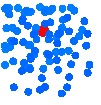
\includegraphics[width=0.25\linewidth]{fig/strategy_1_problem.png}
    \caption{Cod following strategy I in the middle of a school. }
    \label{fig:strat_1_problem}
\end{figure}
This strategy is most commonly exhibited by swordfish and sharks\supercite{pavlov2000behavior}, so is ineffective for the comparatively slower cod. The equation used is below.\supercite{HartonoNguyenTa2024}
\begin{equation}
    F(S,y,v) = -\gamma_1[y-x_{avg}(S)+\gamma_2(v-v_{avg}(S))]\frac{R_2^{\theta_2}}{||y-x_{avg}(S)||^{\theta_2}}
\end{equation}
Initial tests as in Figure \ref{fig:strat_1_problem} show issues with this strategy. Prey are far away enough for avoidance behaviour not to be displayed, and the predator is in the geometric centre of the school, having only captured a few prey in the process. While some of the issues could be solved with improved tuning, Strategy I was therefore not taken further as this behaviour is quite far from that observed.
\subsubsection{Strategy II: Use a weighted average based on distance of fish to calculate the overall force }
\begin{equation}
    F(S,y,v) = -\gamma_1 \sum_{\substack{i=1}}^{N(S)} [y-x_i+\gamma_2(v-v_i)]\frac{R_2^{\theta_2}}{||y-x_i||^{\theta_2}}
\end{equation}
This strategy is most common amongst camouflage fish species\supercite{HartonoNguyenTa2024}. Cod are not camouflage fish, but their ambush strategy is closer to strategy II than strategy I in principle as they also act opportunistically.
\subsubsection{Strategy III: Directly attack the nearest fish}
A third strategy is also considered where cod attack the nearest fish ($n$) in the chosen school by absolute distance. $k$ would also be expected to be close to zero for this strategy, as the effectiveness of this should not change significantly based on school size.
\begin{equation}
    F(y,v,v_n,x_n) = -\gamma_1[y-x_n+\gamma_2(v-v_n)]\frac{R_2^{\theta_2}}{||y-x_n||^{\theta_2}}
\end{equation}
\subsection{Energy}
While generally reaching speeds of up to $1BLs^{-1}$, cod can reach a maximum speed\supercite{Rillahan2008} of up to $5.8BLs^{-1}$. An energy model can therefore be implemented governing the maximum speed of the cod based on distance to prey and current energy $e$, where $0\le e \le 1$.
\begin{equation}
    v_{max} = 0.8+\frac{e}{y-x_{avg}(S)}
\end{equation}
When the cod has run out of energy, it swims at $0.8BLs^{-1}$, still faster than when it is milling. $v_{max}$ is clamped at a maximum of $5.8BLs^{-1}$ regardless of distance and energy.
After any modifications on velocity due to the predator having gone outside the tank walls, the following formula is then applied to the cod's energy.
\begin{equation}
    \frac{de}{dt} = \begin{cases}
    \frac{1}{60}&|v|\le0.5BLs^{-1}\\
    \frac{1}{120}&0.5BLs^{-1}<|v|\le1BLs^{-1}\\
    \frac{1-53^{\frac{|v|}{2L}-\frac{1}{2}}}{3120}&|v|>1BLs^{-1}
    \end{cases}
\end{equation}
This allows the predator to recover all of its energy in 1 minute if milling, or 2 minutes if in the attacking state. The case where $|v|>1BLs^{-1}$ is derived from the following statements\supercite{Rillahan2008}\,\supercite{He1991}:
\begin{enumerate}
    \item Energy cost is exponentially proportional to velocity.
    \item Cod can swim at $3BLs^{-1}$ for a maximum of 1 minute.
    \item Swimming at $\le 1BLs^{-1}$ uses minimal extra energy.
    \item The maximum measured speed is $5.8BLs^{-1}$
\end{enumerate}
The relationship $\frac{de}{dt}=ae^{kv}+c$ can therefore be assumed with the solutions $\left(L, 0\right),\left(3L,\frac{1}{60}\right)$ and $\left(5L,\frac{9}{10}\right)$, where the last solution is an approximation of maximum 6 seconds for the average fish at nearly top speed.
\section{Behaviour optimisation}
To look into what parameters cause optimum performance, an optimisation algorithm is used to tune the chosen parameters ($\alpha, \beta, \gamma$ and $\delta$ for prey, $\gamma_1, \gamma_2$ and $k$ for predators). As prey and predators are optimising for maximum and minimum number of live fish at the end of the simulation, this must be done adversarially, repeatedly alternating which side is being optimised until the total number of alive fish stabilises. 
\subsection{Differential evolution}
Differential evolution (DE) is a genetic optimisation algorithm, where a set of randomly generated samples (population) are modified over generations to maximise a certain output, a process that can be analogised to biological evolution. Below is pseudocode summarising how this works:
\pagebreak
\begin{lstlisting}[language=Python]
const pop_size, max_gen, F, CR, D, bounds
for p in population:
    p.params = sample with random values within the bounds
    p.fitness = run_simulation(p.params)
for generation in range(max_gen):
    for p in population:
        create blank trial
        rand_j = random dimension
        a, b, c = unique population samples chosen randomly
        for dimension j:
            if random(0, 1) < CR or j == rand_j:
                trial[j] = a.params[j]
                + F * (b.params[j] - c.params[j])
                clamp trial[j] to bounds
            else:
                trial[j] = p.prey_vals[j]
        trial_fitness = run_simulation(trial)
        if trial_fitness > p.fitness:
            p = Sample(params = trial, fitness = trial_fitness)        
\end{lstlisting}
The resultant population may not all have similar parameters as different samples may have optimised to different local maximums, and there is no guarantee there is a clear global maximum.
\subsection{Noise reduction}
To reduce the impact of stochastic noise affecting the outcome of a simulation, the total alive fish is the sum over 16 runs using different random seeds.\par
Unreliable strategies would also be worse for the fish as it could cause sudden depletions in the herring population / times when predators are unable to catch herring respectively. To favour more reliable strategies the fitness also penalizes each strategy by half the standard deviation of the number of fish alive.
\subsection{Adversarial}
Much of the research surrounding adversarial implementations of DE is based on Pareto fronts, lines of optimal solutions that maximise parameters that partially conflict. This does not work in the simplified scenario described above, as the optimisations directly contradict each other (with the exception of the above noise reduction).\par
The initial strategy used was to optimise (evolve) the prey over 100 generations, then set the parameters of the prey to the resulting best case, then evolve the predators, and repeat the process. Figure \ref{fig:initial} shows some of the issues with this, where the number of alive fish never stabilises.
\begin{figure}[H]
    \centering
    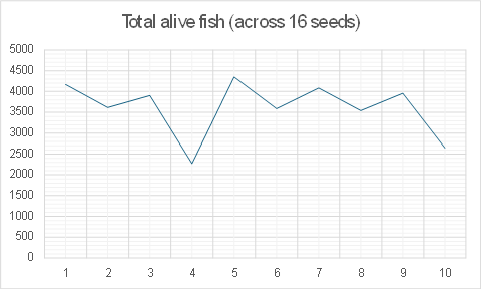
\includegraphics[width=0.5\linewidth]{fig/initial+results.png}
    \caption{Initial results}
    \label{fig:initial}
\end{figure}
\begin{figure}[h]
    \centering
    \begin{subfigure}{0.4\textwidth}
        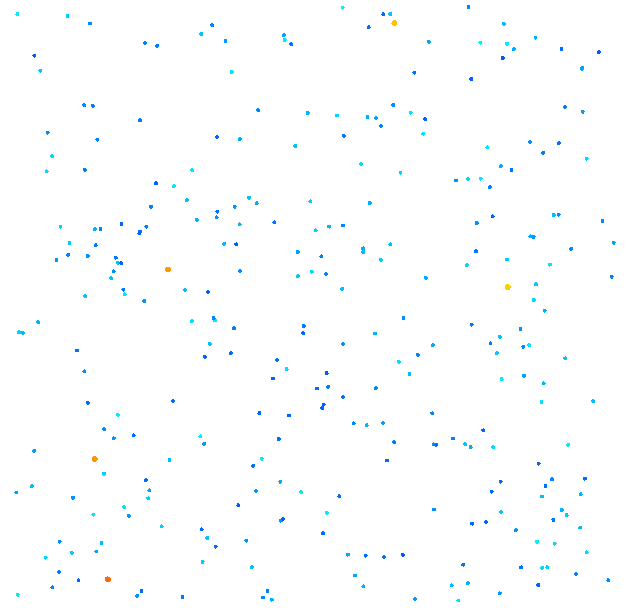
\includegraphics[width=\linewidth]{fig/old_1.png}
        \label{fig:old1}
    \end{subfigure}
    \begin{subfigure}{0.4\textwidth}
        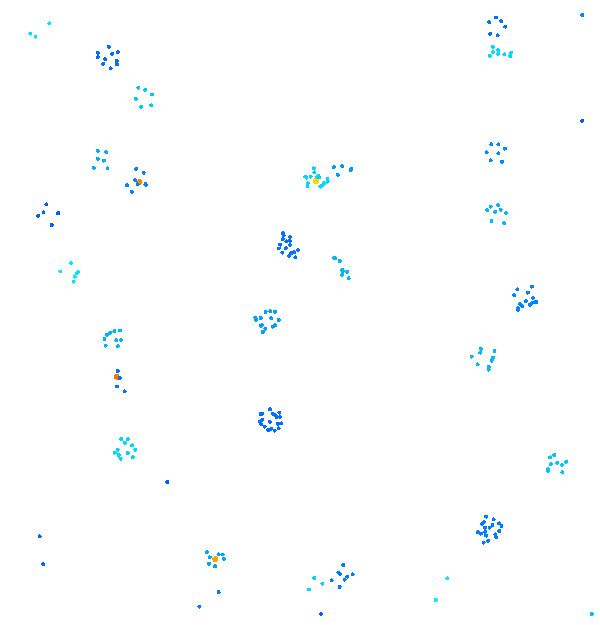
\includegraphics[width=\linewidth]{fig/old2.png}
        \label{fig:old2}
    \end{subfigure}
    \begin{subfigure}{0.4\textwidth}
        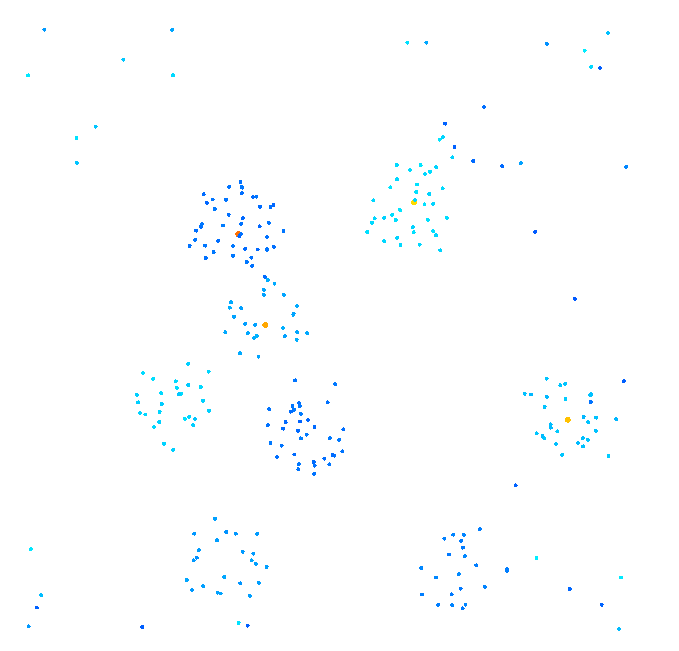
\includegraphics[width=\linewidth]{fig/old3.png}
        \label{fig:old3}
    \end{subfigure}
    \begin{subfigure}{0.4\textwidth}
        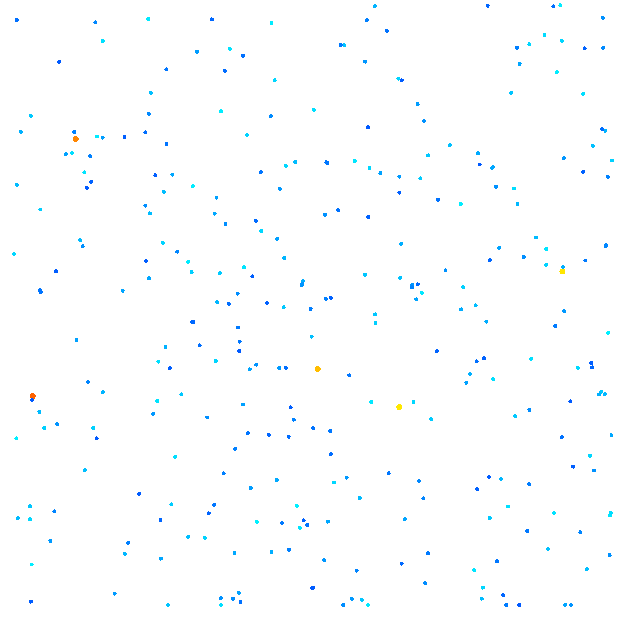
\includegraphics[width=\linewidth]{fig/old4.png}
        \label{fig:old4}
        \end{subfigure}
    \caption{Optimised prey behaviour for the first four iterations.}
    \label{fig:old}
\end{figure}
The reasoning for this lack of converging is clear when each parameter set is visualised, the first four parameter pairs shown in Figure \ref{fig:old}. The pattern of widely spread out $\xrightarrow{}$ very tight schools with non-aligned velocity $ \xrightarrow{}$ loose clumping of schools repeats as the predators optimise to one and the prey change strategy to counteract. \par
This pattern suggests that this method does not work, so a new method of interleaving each mutation was tried, with fitness calculated as the average performance against the 5 best recent opponents within the last 10 generations to prevent overfitting (specialising too much to a single opponent algorithm) by simulating gradual change. These top 5 are referred to as the hall of fame.\par
As the prey and predators are now simultaneously evolving slightly, oscillations are no longer an issue. However, the results are not expected to reach as defined a peak as if only one changed, as evolving both simultaneously effectively means that the landscape where a global maximum (or minimum) needs to be found is constantly shifting. However, the range of values where the peak is still shows what schooling behaviour (or lack of) is being displayed.
\section{Results}

\begin{table}[H]
    \centering
    \begin{tabular}{lcccccccl}
  & \multicolumn{4}{c}{Prey parameters}& \multicolumn{3}{c}{Predator parameters} &Alive\\
          &  $\alpha$&  $\beta$&  $\gamma$&  $\delta$&  $k$&  $\gamma_1$& $\gamma_2$ &\\
          1&  0.3885&  -2.700&  0.3489&  0.000392&  -0.124&  4.803&  1.231&4527\\
          2&  0.25*&  0.25*&  4.892&  0.000465&  0.95&  0.414&  0*&2533\\
          3&  0.355&  -2.627&  2.367&  0.000014&  0.0244&  3.493&  1.467&4375\\
          4&  0.201&  -2.916&  0.851&  0.000633&  0.080&  1.400&  1.197&4575\\
    \end{tabular}
    \caption{Optimised parameters for each simulation condition\\
    * clamped to minimum}
    \label{tab:Results}
\end{table}
\begin{table}[h!]
\centering
\begin{tabular}{ll ll ll ll}
\multicolumn{2}{c}{\textbf{Simulation}} &
\multicolumn{2}{c}{\textbf{Environment}} &
\multicolumn{2}{c}{\textbf{Prey}} &
\multicolumn{2}{c}{\textbf{Predator}} \\
\hline
Population size & 10 & $dt$ & 0.1 & Count & 300 & Count & 5 \\
F & 0.7 & $\sigma$ & 0.2 & $r$ & 0.5 & Vision range & 15 \\
CR & 0.9 & Tank size & 30 & $p$ & 1.5 & Body length & 0.38 \\
Seed count & 16 & Cell count & 10 & $q$ & 2.5 & $R_2$ & 3 \\
Generations& 30& $\epsilon$ & $10^{-6}$ & $a_{\max}$ & 1.5 & $\theta_2$ & 2 \\
HoF count & 5 & $dv$ collision& 0.5 & $v_{\max}$ & 1 & $a_{\max}$ & 0.6 \\
& & & & $v_{\min}$ & 0.03 & & \\
& & & & Vision range & 5 & & \\
& & & & Field of view & $300^\circ$& & \\
& & & & $R_1$ & 3 & & \\
& & & & $\theta_1$ & 1.5 & & \\
\end{tabular}
\caption{Constants}
\label{tab:constants}
\end{table}

Table  \ref{tab:Results} shows the final parameters for the following scenarios. These are taken from the hall of fame, but may not be the best performing parameters as trends across the attempted values were taken into account, as detailed below. Table \ref{tab:constants} shows the constants used\supercite{Giske2008_EmergingSchoolStructures}\,\supercite{HartonoNguyenTa2024}\,\supercite{TaNguyenYagi2017_foraging}.
\subsection{Predator strategy II, no obstacles, no intended clamping of prey parameters}

\begin{figure}[H]
    \centering
    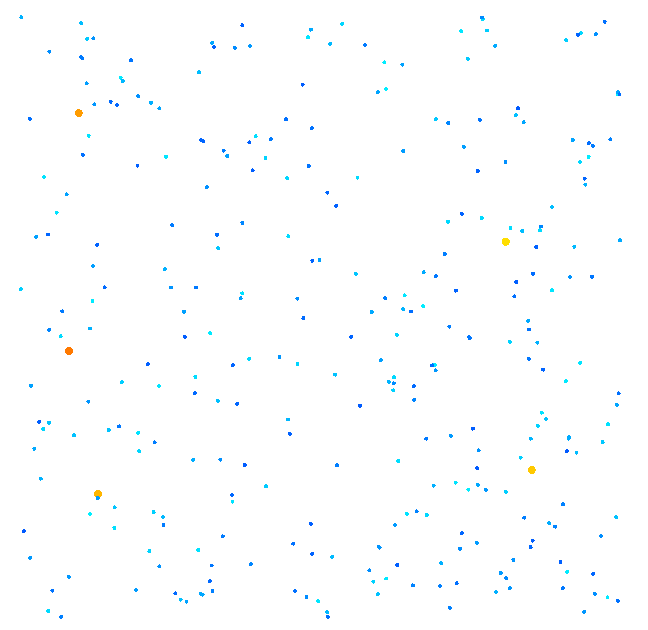
\includegraphics[width=0.5\linewidth]{ii.png}
    \caption{Visualisation of optimal behaviour in the first scenario}
    \label{fig:ii}
\end{figure}
\begin{figure}[H]
    \centering
    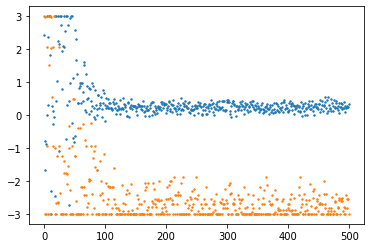
\includegraphics[width=0.5\linewidth]{fig/2-alpha-beta-1.png}
    \caption{$\alpha$ and $\beta$ values tested in each generation}
    \label{fig:a_b_2}
\end{figure}
\begin{figure}[H]
    \centering
    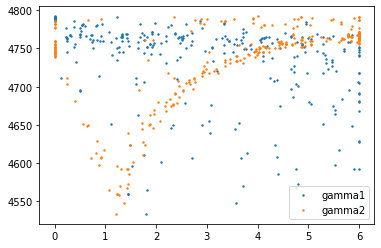
\includegraphics[width=0.5\linewidth]{fig/2_gammas_pred.png}
    \caption{$\gamma_1$ and $\gamma_2$ against number of alive fish (lower means the predator was more successful)}
    \label{fig:2_gammas}
\end{figure}
Figure \ref{fig:ii} shows how the fish behave in this scenario. As $|\beta|>|\alpha|$ and $\beta$ is negative, no schooling behaviour is displayed due to fish moving away from each other. \par
The improvement of the prey to perform better can be seen in Figure \ref{fig:a_b_2}, showing  that $0<\alpha<0.5$ is optimal. With $\gamma_1$ and $\gamma_2$ however, the mutations did not cause the range of possible values to decrease and the hall of fame showed some variance. Plotting $\gamma_1$ and $\gamma_2$ against the number of fish alive at the end of the simulation did however show that the most fish were eaten when $1<\gamma_2<1.5$. This meant that the most reliable parameter set in the hall of fame was likely the best one where this condition is satisfied.\par
Interestingly, plotting the same graph of $\alpha$ and $\beta$ did not yield any more accurate results, suggesting that optimising these parameters past a certain point is impossible due to stochastic noise.
\subsection{Predator strategy II, no obstacles, forced weak schooling behaviour in prey}
\begin{figure}[H]
    \centering
    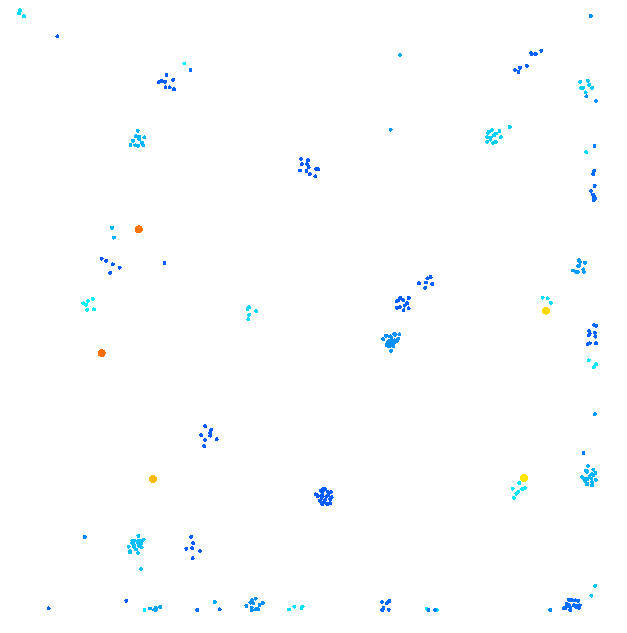
\includegraphics[width=0.5\linewidth]{fig/ii_forced.png}
    \caption{Optimal behaviour for strategy II when schooling is forced}
    \label{fig:2_forced_school}
\end{figure}
This tests predator behaviour and success rate when the herring do school, as shown in Figure \ref{fig:2_forced_school}. As this is not optimal for the prey, the cod perform significantly better than in the first scenario. $\alpha$ and $\beta$ also remained at the set minimum of 0.25, suggesting that there is no local maximum where schooling is beneficial.\par
Predator behaviour also changed significantly in this scenario, with $\gamma_2$ being zero in the entire hall of fame and $k$ being close to 1, showing significant preference towards smaller schools and that velocity matching is not useful.\par
\subsection{Predator strategy II, environmental obstacles of height $h\sim |N(0, 15^2)
|$ }
\begin{figure}[H]
    \centering
    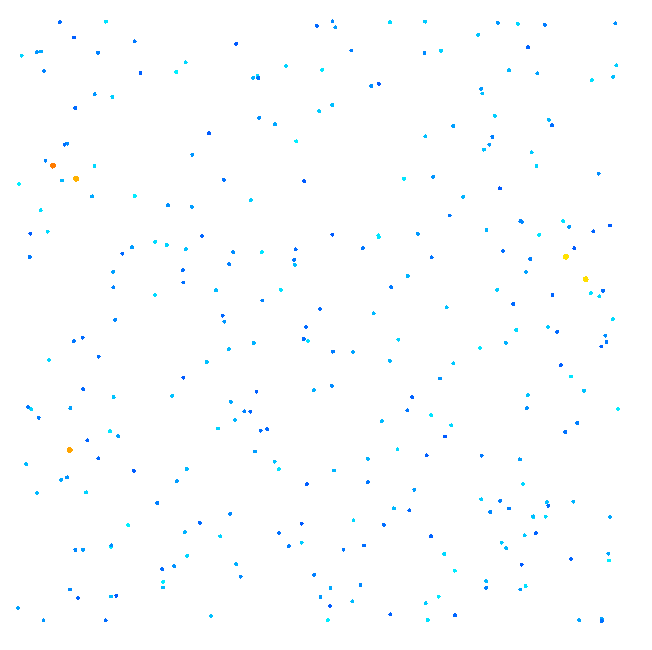
\includegraphics[width=0.5\linewidth]{fig/iii.png}
    \caption{Behaviour in the third scenario}
    \label{fig:scenarioiii}
\end{figure}
\begin{figure}[H]
    \centering
    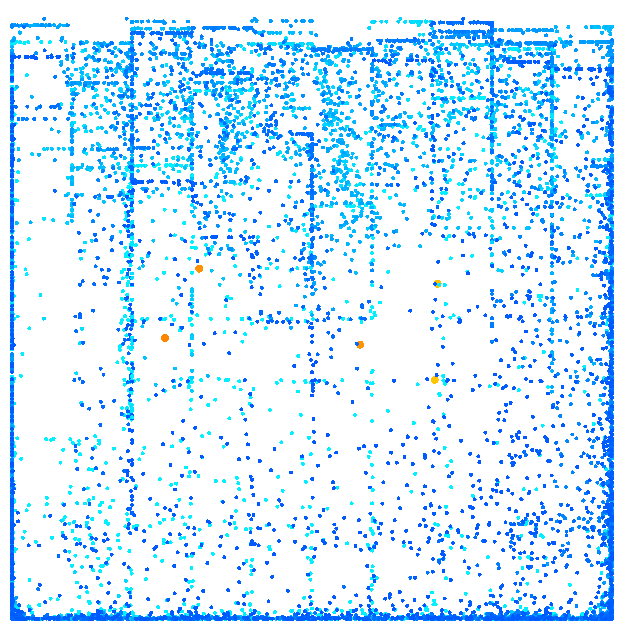
\includegraphics[width=0.5\linewidth]{fig/many_fish.png}
    \caption{10,000 fish with a negative $\gamma$ parameter (attracted to walls), showing obstacles}
    \label{fig:forced walls}
\end{figure}
Figure \ref{fig:scenarioiii} shows the behaviour in this scenario. This looks similar to the first scenario, although the there is an increase in density of herring at the bottom of the image as there are no obstacles here\footnote{Due to the lack of transformations in the visualisation and defining the bottom of the tank as zero, this appears inverted}. The position of obstacles is not obvious in the visualisation as they are transparent to ensure all fish are visible, but Figure \ref{fig:forced walls} shows their position.\par
The values in this scenario were very similar to that of the first, although the graphs produced show greater variance, likely explaining the change in $\delta$ (the variable with the weakest observed correlation). $\gamma$ is higher in this, likely due to the higher chance of collision meaning avoidance is more important.
\subsection{Predator strategy III, no obstacles, no intended clamping of prey parameters}
\begin{figure}[H]
    \centering
    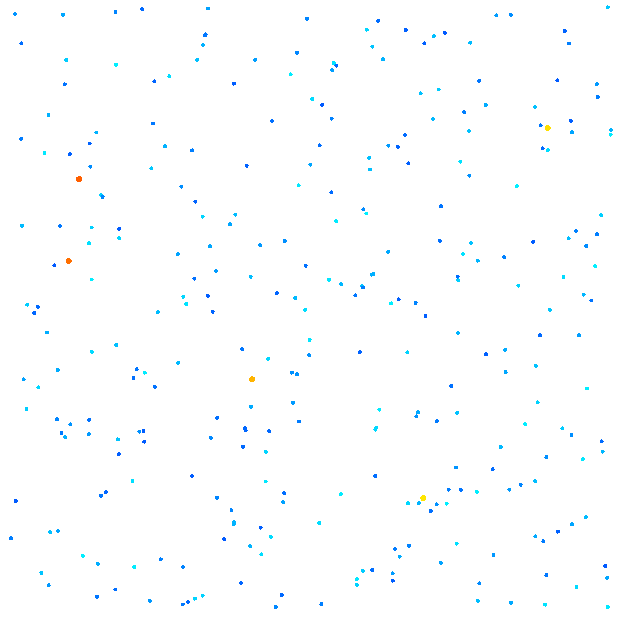
\includegraphics[width=0.5\linewidth]{fig/scenario4.png}
    \caption{Behaviour for the fourth scenario}
    \label{fig:scenarioiv}
\end{figure}
\begin{figure}[H]
    \centering
    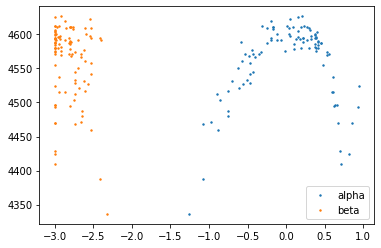
\includegraphics[width=0.5\linewidth]{fig/alpha_beta.png}
    \caption{$\alpha$ and $\beta$ against alive fish (higher means prey were more successful)}
    \label{fig:alphabeta}
\end{figure}
Figure \ref{fig:scenarioiv} shows the behaviour with this strategy. Both the appearance and parameters in this are quite similar to the first and third scenario, aside from $\gamma_1$ being closer to $\gamma_2$, meaning velocity matching is more important here. Figure \ref{fig:alphabeta} shows a defined maximum for $\alpha$ however, unlike in any of the other optimisations.
\section{Conclusion}
The results of this simulation are unexpected: schooling, a known defence mechanism, is not optimal for surviving cod attacks. The extent of this does not significantly change depending on predator strategy or obstacles, although herring performance does vary. The parameters for cod change more significantly depending on the scenario, although this may be partially accounted for by the higher variance in the hall of fame.\par
Given Figures \ref{fig:alphabeta} and \ref{fig:2_gammas} show clear maximum / minimums, it is evident that these parameters are possible to optimise, although the amount of noise mean that doing so accurately is not possible without significantly more generations and iterations of the simulation with different random seeds, as well as simulating over a longer time period.\par
The tendency away from schooling may be due to the constraints of the model. The number of predators and prey is very small, so schooling benefits are not observed as much. There are also many other factors this model does not take into consideration, such as feeding behaviour of herring, other predators and hydrodynamic benefits of schooling\supercite{shaw1978schooling}. A more sophisticated model on a larger scale would be required to confirm this.
\section{Evaluation}
I chose this project because I am interested in how inspiration is taken from nature to write algorithms for swarm robotics. Given that I did not have the time to build physical devices I decided to use the constraints of an animal. When deciding on the details, I ended up removing the robotics element entirely as I wanted to explore adversarial algorithms. This meant that the project became closer to computational biology than intended, which presented its own challenges as I have no intuition for how herring would behave. The result of this is that I am unsure as to how good my results are, as (for understandable reasons) there have not been experimental studies with conditions similar to those simulated.\par
A secondary aim for this project was to learn C++, as I wanted to do so over the summer anyway. As a result, my code is more inconsistent and inefficient than usual. This was definitely not the easiest first program to write in C++, as I spent a lot of time trying to debug issues that I had never come across in other languages. However, there were many benefits, such as being able to use all 16 cores at 100\% (hard in Python due to the global interpreter lock). This project forced me to understand C++ in more depth than I would have needed if I had written something where performance did not matter, which I am very glad about.\par
Given my uncertainty of the success of the individual results, the aspect that I am using to measure my success is the methodology. Adversarial differential evolution has not been used in predator-prey simulations before, and the graphs do show a defined (albeit noisy) maximum, suggesting that this is a valid method. I have also added onto the published SDEs with constraints such as energy budgets. This was mostly done through reading ecology papers, which was far more interesting than I initially expected.
\section{Appendix}
The simulation and analysis code, as well as the \LaTeX\ source for this document, can be found on GitHub, at https://github.com/ice-cube-1/herring-1/.
\printbibliography
\end{document}
